\lecture{7}{Feb 3 10:10}{}
\[
    \Delta = q \Delta \phi 
\]
\[
    \phi (\vec{r} ) = \phi (\vec{r} _0) + \Delta \vec{r} \cdot \nabla  \phi \at{}r = r_0{}{} 
    + \frac{1}{2} (\Delta \vec{r}  )
\]

For the first condition we have 
\[
    E (\vec{r} )= 0 
\]

For the second condition we have 
\[
    \Delta \phi  > 0
\]
for all directions 
\[
     \Delta = \Delta y = \Delta z
\]
\[
    \left(  \frac{\partial ^{2} }{\partial x ^{2} } + 
    \frac{\partial ^{2} }{\partial y ^{2} } + 
    \frac{\partial ^{2} }{\partial z ^{2} } + 
    \right) \phi  > 0
\]
\[
    \nabla ^{2}  \phi  = - \frac{\rho}{\epsilon } > 0\implies  \rho (\vec{r} ) \neq  0 
\]
If we assume that \(\rho = 0\). At least one of the directions should have the derivative 
\[
    \frac{\partial ^{2}  \phi }{\partial j ^{2} } < 0 
\] 
\begin{figure}[H]
    \centering
    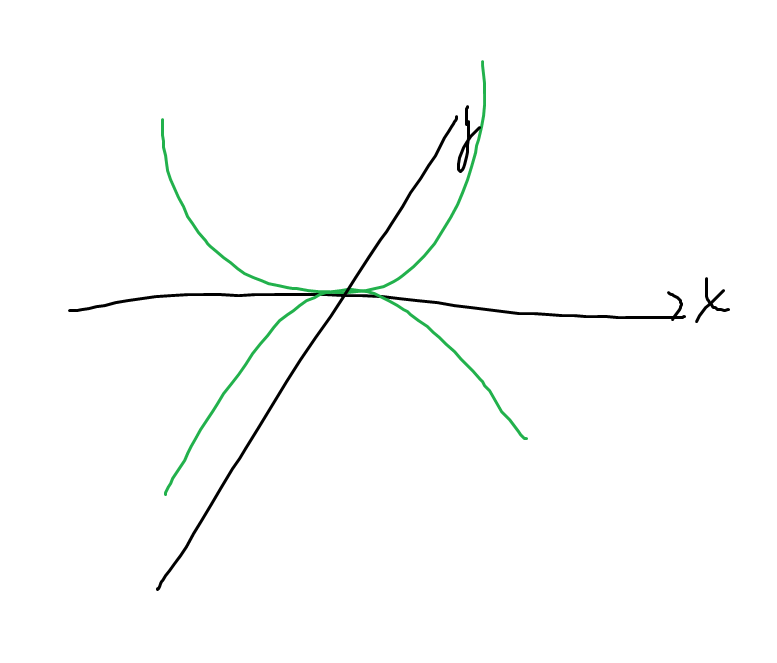
\includegraphics[width=0.8\textwidth]{Figures/02.png}
    \caption{}
    \label{fig:}
\end{figure}
\paragraph{Trapped Ions}
\begin{eg}
This is useful for trapped ion quantum computing. There are two ways to hold a ion they use something 
called a Paul trap which uses a set of electrodes and alternates the electrodes which causes a rotating 
electric field or (AC field). This creates a quadruple moment which creates a trap in 3D. 

The other method is called the \textbf{penning trap}  where there is a static \(\vec{E} \)  field 
and a \(B\)  field in the \(z \)  direction. 
\end{eg}

\paragraph{Electrostatics for atoms, molecules, molecules, and crystals}
\begin{eg}

    For the classical pictures of atoms (hydrogen atom), we have the following 

    \begin{figure}[H]
        \centering
        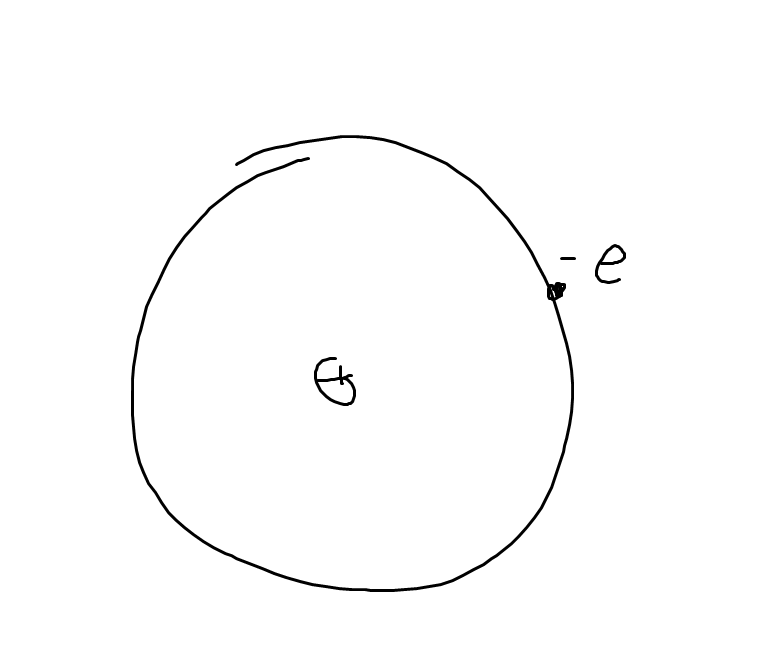
\includegraphics[width=0.8\textwidth]{Figures/03.png}
        \caption{}
        \label{fig:}
    \end{figure}
    
    \[
        U = U_k + U_p
    \]
    which is the total energy (kinetic and potential)
    \[
        U_k = \frac{1}{2} m v ^{2} 
    \]
    or defined in terms of angular momentum to be 
    \[
        \frac{L^{2} }{2mR^{2} }
    \]
    The potential energy is going to be 
    \[
        U_p = \frac{-q_e q_p}{4\pi \epsilon _0 R}
    \]
    Additionally, Bohr Postulates that 
    \[
        L = n \hbar 
    \]  
\end{eg}

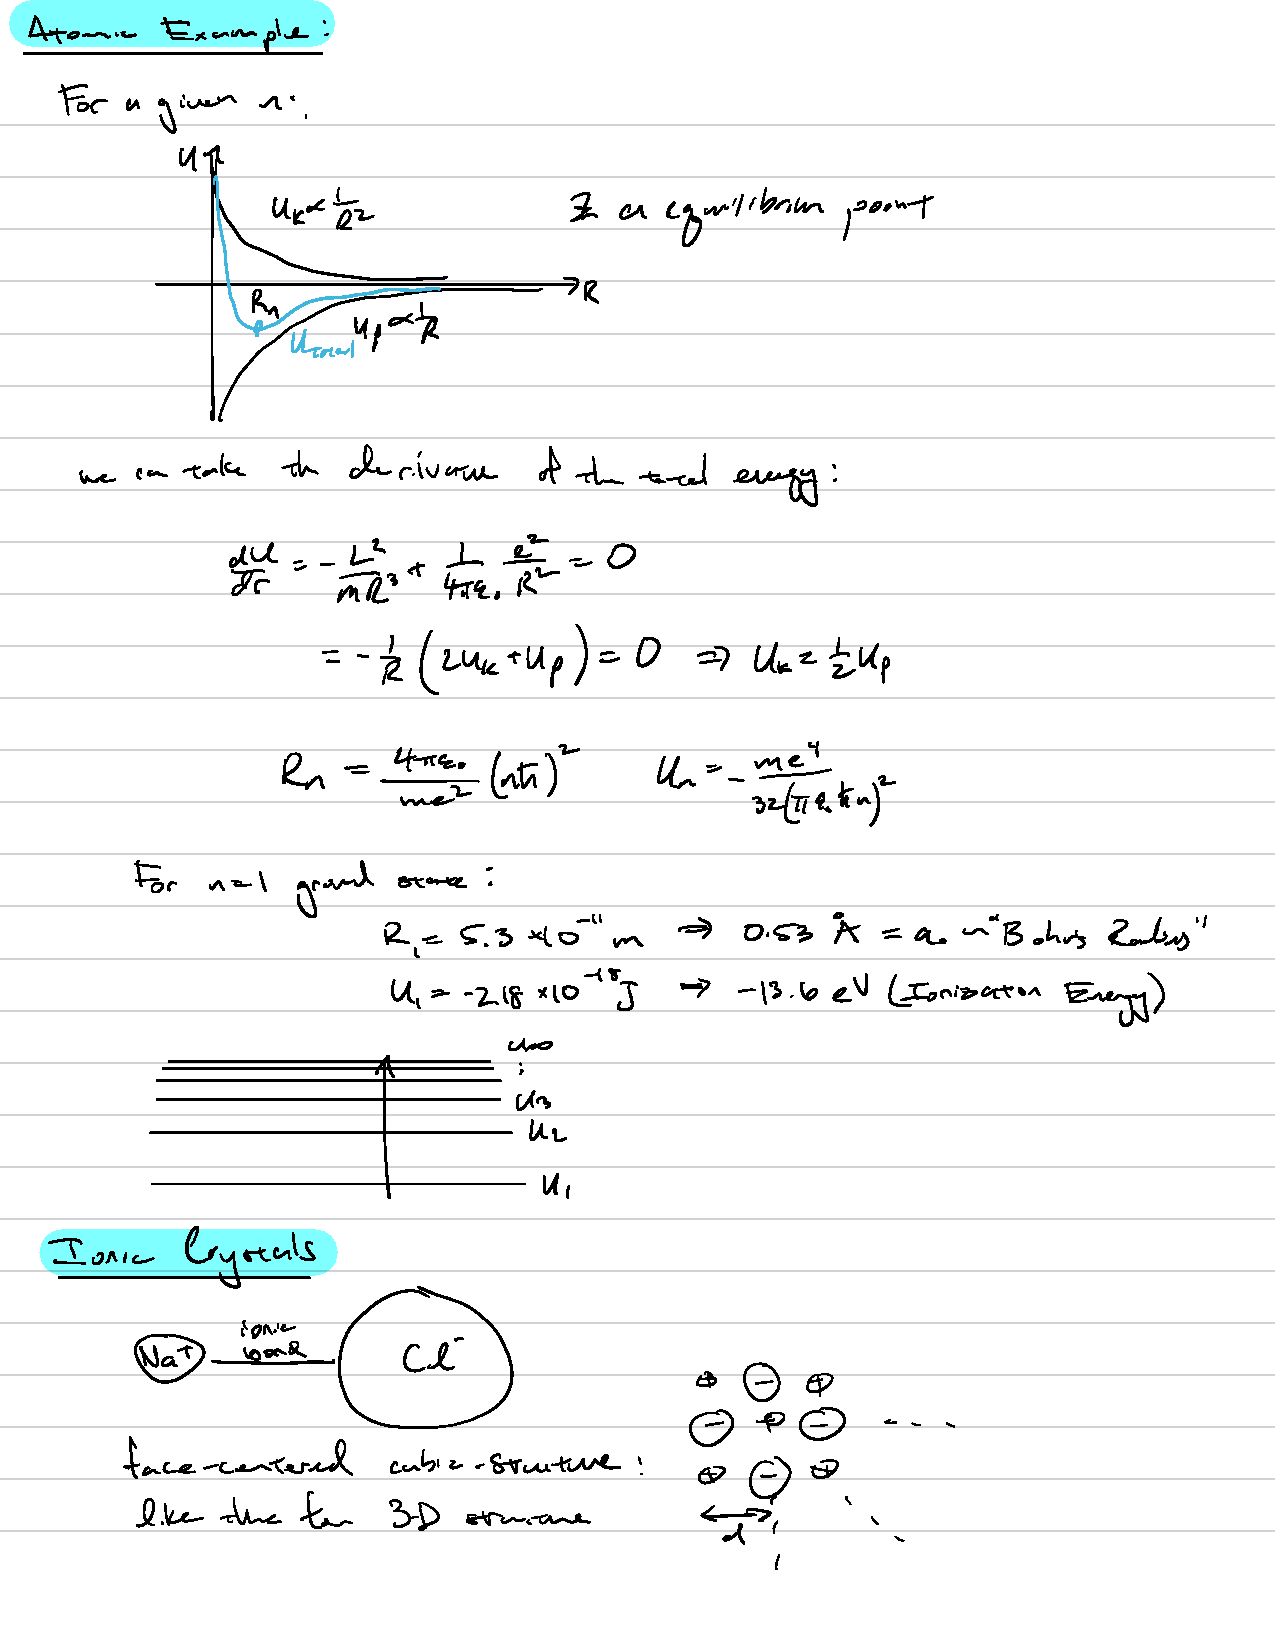
\includepdf[pages=-]{"Lectures/lec7.pdf"}
